\documentclass[a4paper,12pt]{article}

%% Language and font encodings
\usepackage[english]{babel}
\usepackage[utf8x]{inputenc}
\usepackage[T1]{fontenc}

%% Sets page size and margins
\usepackage[a4paper,top=3cm,bottom=2cm,left=3cm,right=3cm,marginparwidth=1.75cm]{geometry}

%% Useful packages
\usepackage{amsmath}
\newcommand{\norm}[1]{\left\lVert#1\right\rVert}
\usepackage{amssymb} 
\usepackage{graphicx}
\usepackage[colorinlistoftodos]{todonotes}
\usepackage[colorlinks=true, allcolors=blue]{hyperref}
\usepackage{dsfont}

%% Manual Operators 
\DeclareMathOperator*{\argmin}{arg\,min}
\DeclareMathOperator*{\argmax}{arg\,max}

\title{ML HW 2}
\author{Karl Jiang}


\begin{document}
\maketitle 


\section{Support Vector Machines}

\subsection{Problem 1: Quadratic Programming} 

After some math, the lecture can express the optimization problem above with the objective as: 

$$
\textrm{max} \bigg\{ \sum_{i=1}^N \alpha_i - \frac{1}{2} \sum_{i,j=1}^N \alpha_i \alpha_j y_i y_j K(\mathbf{x_i, x_j}) \bigg\} 
$$

Subject to the constraints: 

$$
\sum_{i=1}^N \alpha_i y_i = 0, 0 \leq \mathbf{\alpha} \leq C
$$

Which is equivalent to

$$
 \textrm{min} \bigg\{ -\sum_{i=1}^N \alpha_i + \frac{1}{2} \sum_{i,j=1}^N \alpha_i \alpha_j y_i y_j K(\mathbf{x_i, x_j}) \bigg\} 
$$

Let's start with the objective: 

$$
\mathbf{\alpha^T H \alpha + f^T\alpha} = \sum_{i,j = 1}^N \alpha_i \alpha_j H_{ij} + \sum_{i = 1}^N f_i \alpha_i  
$$

Then, $H_{ij} = y_i y_j K(\mathbf{x_i, x_j})$, so $\mathbf{H = yy^T \circ K}$ where $\mathbf{K}$ is the matrix with entries $K_{ij} = K( \mathbf{x_i, x_j} )$ 
, and $f_i = -1 \implies \mathbf{f} = \mathbf{-1}$ the length n vector with entries -1.

$\\$
Inequality Contraint: 
$$ 
0 \leq \mathbf{\alpha} \leq C \implies 
0 \leq \alpha_i \textrm{ and } \alpha_i \leq C 
$$

So for each $\alpha_i$, there are two constraints. In total then, there are $k_{inequal} = 2n$ constraints. 
If we define $\mathbf{a}$ to be the length $2n$ vector
$$
\mathbf{a} = 
\begin{bmatrix} 
	0 \\
	\vdots \\
	0 \\
	C \\ 
	\vdots \\ 
	C 
\end{bmatrix} 
$$

with $\mathbf{a_{1:n}} = 0$ and $\mathbf{a_{n+1:n}} = C$, then we can define 

$$
\mathbf{A}_{2n x n} = 
\begin{bmatrix} 
	-I_{nxn} \\
	 I_{nxn} \\
\end{bmatrix} 
$$

To express the inequality constraints $ \mathbf{A \cdot \alpha \leq a}$. 

$\\$

Equality Constraint: 

Here we only have $k_{eq} = 1$ constraint. We then have 
$$
\sum_{i = 1}^N y_i \alpha_i = 0 
\implies \mathbf{y^T\alpha} = 0 
\implies \mathbf{B_{1xn} = y^T} \textrm{, } \mathbf{b_{1x1}} = 0 
$$

To satisfy the constraint $\mathbf{B \cdot \alpha = b}$

$\\\\$
In summary: 

$
\\ 
\mathbf{H = yy^T \circ K} \\ 
\mathbf{f = -1} \\
\mathbf{A}_{2n x n} = 
\begin{bmatrix} 
	-I_{nxn} \\
	 I_{nxn} \\
\end{bmatrix} \\ 
\mathbf{a_{2n}} = 
\begin{bmatrix} 
	a_1 \\
	\vdots \\
	a_n \\
	a_{n+1} \\ 
	\vdots \\ 
	a_{2n} 
\end{bmatrix} 
= 
\begin{bmatrix} 
	0 \\
	\vdots \\
	0 \\
	C \\ 
	\vdots \\ 
	C 
\end{bmatrix} \\
\mathbf{B_{1 x n} = y^T} \\
\mathbf{b_{1 x 1}} = 0  
$ 




\section{Decision Trees} 

\subsection{Problem 3: Linearly seperable} 

If the data is linearly seperable, we are able to perfectly classify the N points using the decision tree. This is just the simple case of severely overfitting onto the training data by having one leaf / region for each data point ($N$ leaves / regions). In the best case scenario, only two leaves are required (eg. the data can be perectly split on an axis parallel to x1 or x2). 

$\\$
The depth of the tree is then, in the best case scenario, 1. (1 split). If we add points according to this rule, we will still only require two leaves / regions, and therefore the depth will remain 1, and is independent of the number of samples. Hence the depth in the best case for linearly separable data is $O(1)$.  

$\\$
In the worst case scenario, consider the line $x_2 = x_1$, shown below, where positive classes lie on a line slightly above and parallel to the separating hyperplane, and slightly below for negative classes. 

\begin{figure}[h!]\centering%{width=4.0in}
	\caption{\textbf{Linear 45}}\label{FigExample}
	    \fbox{\resizebox{4.0in}{3.0in}{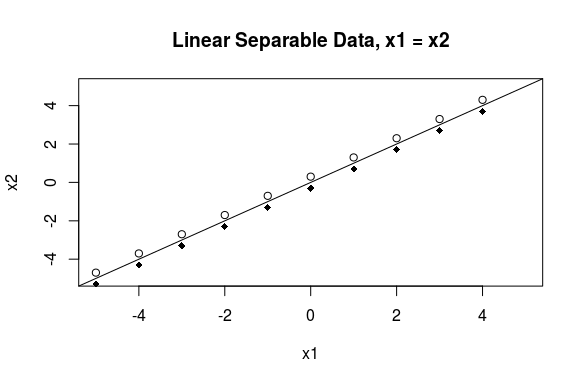
\includegraphics{linear}}}
\end{figure}

By CART, gini loss is minimized by creating a region around one point at each step, giving us the worst case scenario $N$ leaves. This will result in a depth that scales linearly with $N$. Thus, the worst case scenario is $O(N)$.   

\subsection{Problem 4: Nonlinear seperable} 

Again, we can perfectly classify the $N$ points with $N$ leaves, assuming that no two points that have different classes share the same cordinates. 

$\\$
Best case scenario: Consider all positive classes on the line $x_2 = 0$, and negative classes on the line $x_2 = 1$ and $x_2 = -1$. 

\begin{figure}[h!]\centering%{width=4.0in}
	  \caption{\textbf{NoneLinear 2 Regions}}\label{FigExample}
	    \fbox{\resizebox{4.0in}{3.0in}{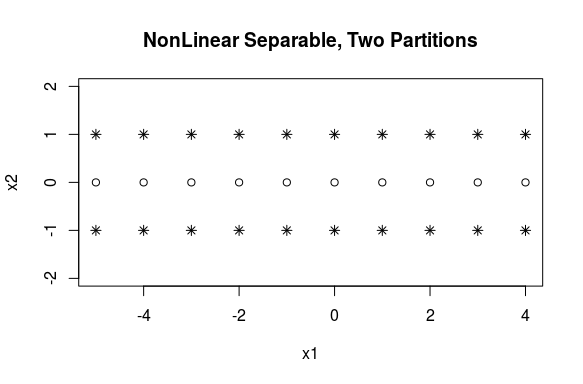
\includegraphics{nonlinear_O1}}}
\end{figure}

Here, only two partitions are required: one between (0,1) and in (-1,0). Here we have a depth of two. Note that it doesn't matter how many samples there are according to this rule. Thus, the base case has a depth $O(1)$. 

$\\$
Worst Case Scenario: Consider alternating classes on the line parallel to $x_1$. By CART, gini impurity is minized by classifying one point correctly (either far left or far right point) at each step until all points are perfectly classified. This results in a tree with a depth that scales linearly with $N$ as we will have $N$ leaves with a new leaf node at each step. Hence, the worst case is $O(N)$. 

\begin{figure}[h!]\centering%{width=4.0in}
	  \caption{\textbf{Nonlinear N Regions}}\label{FigExample}
	    \fbox{\resizebox{4.0in}{3.0in}{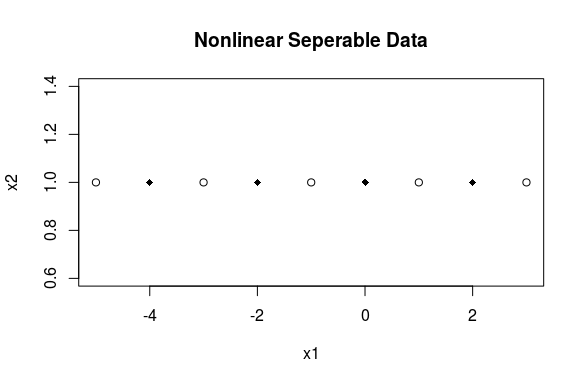
\includegraphics{nonlinear}}}
\end{figure}


\section{Boosting} 


\subsection{Problem 5} 

Let the training error of $h_{T+1}$ under the new weights be $\epsilon_{T+1}'$ and the sum of the updated weights (the normalization constant) be $Z^{t+1}$ Then we have:   

$$
\begin{aligned} 
	\epsilon_{T+1}' &= 
	\sum_{i: y_i \neq h_{t+1}(x_i) }^N W_i^{t+1} \\ 
	&= \sum_{i: y_i \neq h_{t+1}(x_i) }^N
	\frac{1}{Z^{t+1}} W_i^{t} e^{
		-\alpha_{t+1}y_ih_{t+1}(\mathbf{x_i}) } \\
	&= \frac{e^{\alpha_{t+1}}}{Z^{t+1}} 
	\sum_{i: y_i \neq h_{t+1}(x_i) }^N W_i^t \\
	&= \frac{e^{\alpha_{t+1}} \sum_{i: y_i \neq h_{t+1}(x_i) }^N W_i^t}{\sum_{i = 1 }^N W_i^{t} 
		e^{-\alpha_{t+1}y_ih_{t+1}(\mathbf{x_i}) } } \\ 
	&= \frac{e^{\alpha_{t+1}} \sum_{i: y_i \neq h_{t+1}(x_i) }^N W_i^t}
	{e^{\alpha_{t+1}}\sum_{i: y_i \neq h_{t+1}(x_i)}^N W_i^t + e^{-\alpha_{t+1}}\sum_{i: y_i = h_{t+1}(x_i)}^N W_i^t }  \\ 
\end{aligned} 
$$

Now we use the fact that that the weights sum to one: $\sum_{i=1}^N W_i^{t} = 1$ at each step and that $\epsilon_{t+1} = \sum_{i: y_i \neq h_{t+1}(x_i)}^N W_i^t$. We also use the fact that $\alpha_{t+1} = \frac{1}{2} \textrm{log}( \frac{1 - \epsilon_{t+1}}{\epsilon_{t+1}} ) $ 

$$
\begin{aligned}
    &\implies \frac{e^{\alpha_{t+1}} \sum_{i: y_i \neq h_{t+1}(x_i) }^N W_i^t}
	{e^{\alpha_{t+1}y_ih_{t+1}(\mathbf{x_i}) } \sum_{i: y_i \neq h_{t+1}(x_i)}^N W_i^t + e^{-\alpha_{t+1}y_ih_{t+1}(\mathbf{x_i}) } \sum_{i: y_i = h_{t+1}(x_i)}^N W_i^t } \\
    &= \frac{e^{\alpha_{t+1}} \epsilon_{t+1} }{ e^{\alpha_{t+1}} \epsilon_{t+1} + e^{-\alpha_{t+1}} (1 - \epsilon_{t+1} ) } \\
    &= \frac{e^{2\alpha_{t+1}} \epsilon_{t+1} }{ e^{2\alpha_{t+1}} \epsilon_{t+1} + 1 - \epsilon_{t+1}} \\
    &= \frac{ \frac{1 - \epsilon_{t+1}}{\epsilon_{t+1}} \epsilon_{t+1}}{\frac{1 - \epsilon_{t+1}}{\epsilon_{t+1}} \epsilon_{t+1} + 1 - \epsilon_{t+1}} \\ 
    &= \frac{1 - \epsilon_{t+1}}{1 - \epsilon_{t+1} + 1 - \epsilon_{t+1}} \\ 
    &= \frac{1}{2} 
\end{aligned} 
$$

Can we select the same classifier again? That would mean the weighted training error, as we have shown about, would be 
$\epsilon_{t+1}' = \frac{1}{2}$. Then the weight of the classifier would be 
$\alpha_{t+1}' = \frac{1}{2} \textrm{log}(\frac{1 - \epsilon_{t+1}'}{\epsilon_{t+1}'}) = \frac{1}{2}\textrm{log}(1) = 0$, so using the same classifier would be pointless as its classification would not considered in $H_{t+1}(\mathbf{x_i})'$. 

\subsection{Problem 6}

The we take the gradient of the loss $L(\mathbf{X, y})$ at iteration $t$ with respect to $\alpha_t$. Assuming that the weights sum up to each iteration, we have: 

$$
\begin{aligned} 
	L &= \sum_{i=1}^N W_i^{t-1}e^{-\alpha_t y_i h_{t}(\mathbf{x_i})} \\
	&= e^{\alpha_{t}}\sum_{i: y_i \neq h_{t}(x_i)}^N W_i^t + e^{\alpha_{t}}\sum_{i: y_i = h_{t}(x_i)}^N W_i^t \\ 
	&= e^{\alpha_{t}}\epsilon_{t} + e^{-\alpha_{t}}(1 - \epsilon_{t})  
\end{aligned} 
$$

Giving us a gradient: 

$$
\begin{aligned}
	\frac{\partial L}{\partial \alpha_t} &= -e^{-\alpha_{t}}(1 - \epsilon_{t}) + e^{\alpha_{t}}\epsilon_{t} 
\end{aligned} 
$$

Setting to zero to find the critical point: 

$$
\begin{aligned}
	&\implies \frac{\partial L}{\partial \alpha_t} = 0 \\
	&\implies e^{-\alpha_{t}}(1 - \epsilon_{t}) + e^{\alpha_{t}}\epsilon_{t} = 0 \\ 
	&\implies e^{2\alpha_{t}}\epsilon_{t} = (1 - \epsilon_{t}) \\
	&\implies 2\alpha_t = \textrm{log}(\frac{1 - \epsilon_t}{\epsilon_t}) \\
	&\implies \alpha_t = \frac{1}{2} \textrm{log}(\frac{1 - \epsilon_t}{\epsilon_t})
\end{aligned} 
$$

The second dervative will yield the original loss function which is positive for all values of $\alpha_t$, thus the loss function achieves a minimum at this point, that is $\alpha_t = \frac{1}{2} \textrm{log}(\frac{1 - \epsilon_t}{\epsilon_t})$ minimizes the empirical loss. 

\subsubsection{Credits} 

The great Julian McClellan and Isaac Adeleke. 

\end{document}


